\chapter{System Requirements and Specification}

\section{Description}
Throughout the following chapter, the system designs of the project will be represented as diagrams. Using use-case diagrams, Activity diagrams and sequence diagrams with descriptions of these such diagrams displayed throughout the chapter as an aid in understanding the communications between each specific component of the app. These are needed for the reader to be able to comprehend the app as a whole. 

\section{Underlying Architecture of the Android OS}
Regarding the underlying architecture on which an application will be in fact lying on top of the Android operating system. The following operating system is, in fact, a stack of software components which are mapped in coordinance with the corresponding hardware modules at the Linux kernel layer. The software stack is roughly divided into five specific sections and four different layers of which the frameworks, libraries, kernel and applications sit. The following diagram in figure 5.1 shows this. 

\begin{figure}[htbp]
    \center 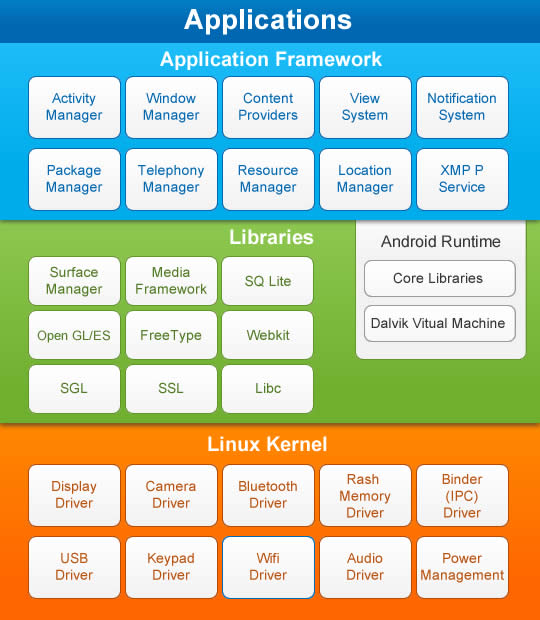
\includegraphics[width=400pt]{AndroidOS}\\
    \caption{Android Architecture \citep{androidlife}} \label{Figure: Android Architecture}
\end{figure}
\par 
Concerning the Linux layer of the following OS. The version of which is Linux 3.6 on which has approximately 115 patches to its name. This layer acts as a level of abstraction between the devices software modules and its hardware components on which contains the following, camera module, keypad, display, GPS and a wifi module, etc. Utilising the fact that Linux is a great source for networking and on which supports a vast array of drives which provided a solid base on providing a somewhat reliable OS.

\section{Android's Incorporated libraries}
Concerning the libraries of which are incorporated within the application these apps are used to retrieve information on which may be related to specific applications on the device. On top of the Linux kernel, there are a set of libraries which includes an open source web engine WebKit, libc which is a standard C library which was created by Google for its Android OS and also an SQLite database of which is a useful repository for storage and sharing of application data throughout the program. Other libraries also include SSL which is responsible for the security of the device with regards to internet connectivity. Other libraries are also included to record and play audio and video.
\section{A Look at Android's Location Service's}
Utilising a client's mobile device on gaining their exact location can be done in two ways one of which is favoured over the other. The first way of allocating the user's location can be done by utilising the GPS module of the device by using Android's built-in Location API's which have been available since Android's first launch. These location gathering API's still work even to this day. However, uses a lot of the device's power to gain specific coordinates. With the following in mind, the user must more likely be outdoor's for the following to work to get a signal to a GPS satellite.

\paragraph{Google Play Services} -
The developer of the application InforMe@Dublin has utilised a new way of gaining clients geographical coordinates by way of using Google Play Services of which provides a very powerful, high-level framework to work from. This provides a choice of location gathering tools, such as WIFI and internet connection, GPS modules, cellular fixation or to bundle these together to provide a more accurate location fixture. The following API allocates power management of the device to keep each mobile phone at the top of its game.
\par
Android gives applications of which access location services supported by the device through classes in the android.location package. The most important component of the following framework is the LocationManager which is a system service related to figure 5.1. The following provides APIs for determining the location of which the device is in at that current time. The digram located in figure 5.2 shows how the location service and manager work together with the system in order to retrieve the devices location.

\begin{figure}[htbp]
	\center 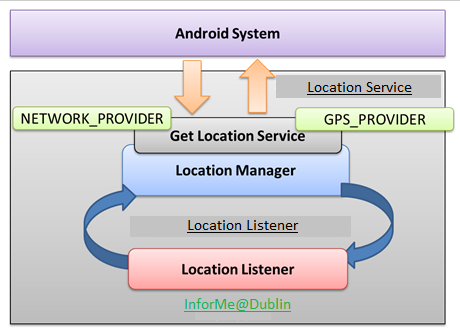
\includegraphics[width=400pt]{locationManager}\\
	\caption{Retrieving Location} \label{Figure: Retrieving Location}
\end{figure}


\section{Installation of InforMe@Dublin}
Before the user accessing the following application, the app may first be downloaded from the Google play store on which the developer has chosen to release to the general public. The application would be available or work for people living in the Dublin area. When the application has been downloaded and of the installation being completed the following diagrams will show how the system works.

\section{Login and Authentication Diagrams}
The following diagrams represent the application's login page as well as some various activities on which the user may enter before moving forward while using the application.

\subsection{Login Use Case Diagram}
Regarding the Use Case diagram in figure - 5.3, The reader can grasp the associated activities that are compiled within the login page. When first starting the InforMe@Dublin application the user may only use the following activities to gain access to the map area of that app. Which are Google sign in, Creation of an account, forgotten password of an existing account or to log in with the user's credentials if account already created.\par

\begin{figure}[htbp]
    \center 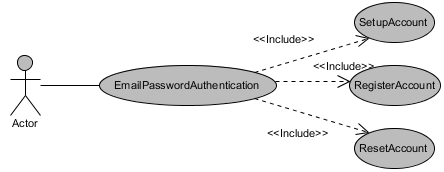
\includegraphics[width=450pt]{EmailAndPasswordUsecase}\\
    \caption{Login Use case Diagram} \label{Figure: Login Use case Diagram}
\end{figure}

\subsection{Login Activity Diagram}
Regarding the following Activity Diagram in figure - 5.4, The developer has produced an activity diagram displaying how each component works with one another. As the following classes and activities are seen is how the source code is laid out. Each specific part of the Android app has its specific package for the purpose of modularity. While visualising the diagram the reader can distinguish how each of the specific button clicks are mapped. Each specific activity has its very own methods on which the user must specifically progress through to gain access to the signed in activities these specific buttons and menus are hidden until the client has been authenticated by firebase's authentication method which is located in the EmailPasswordAuthentication activity.
\begin{figure}[htbp]
    \center 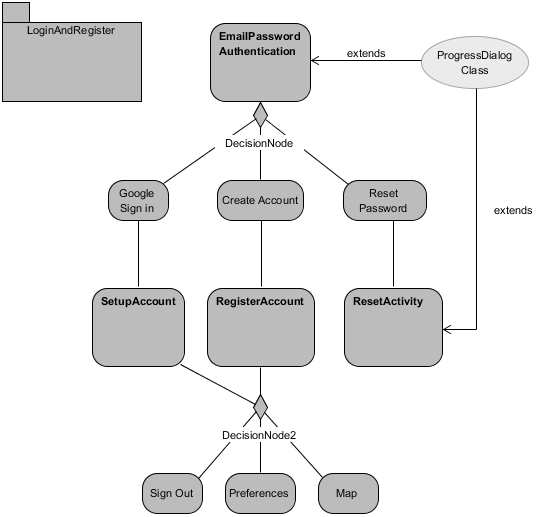
\includegraphics[width=450pt]{Login&RegisterActivity}\\
    \caption{Login Activity Diagram } \label{Figure: Login Activity Diagram}
\end{figure}

\subsection{Login Sequence Diagram}
Regarding the sequence diagram located in figure 5.5, The Reader can comprehend what tasks are being processed in the background by their actions on which they are pursuing. While starting the application and looking at the following diagram the reader can see the generic association between the actor and the EmailAndPasswordAuthentication activity which is created on starting the app. Which checks immediately if a user was already signed in using the mobile device and have not specifically signed out which allows the user to access a new set of activities which enable them to discover Dublin in a new light and to find hidden monuments that have stood the test of time.\par

\begin{figure}[htbp]
    \center 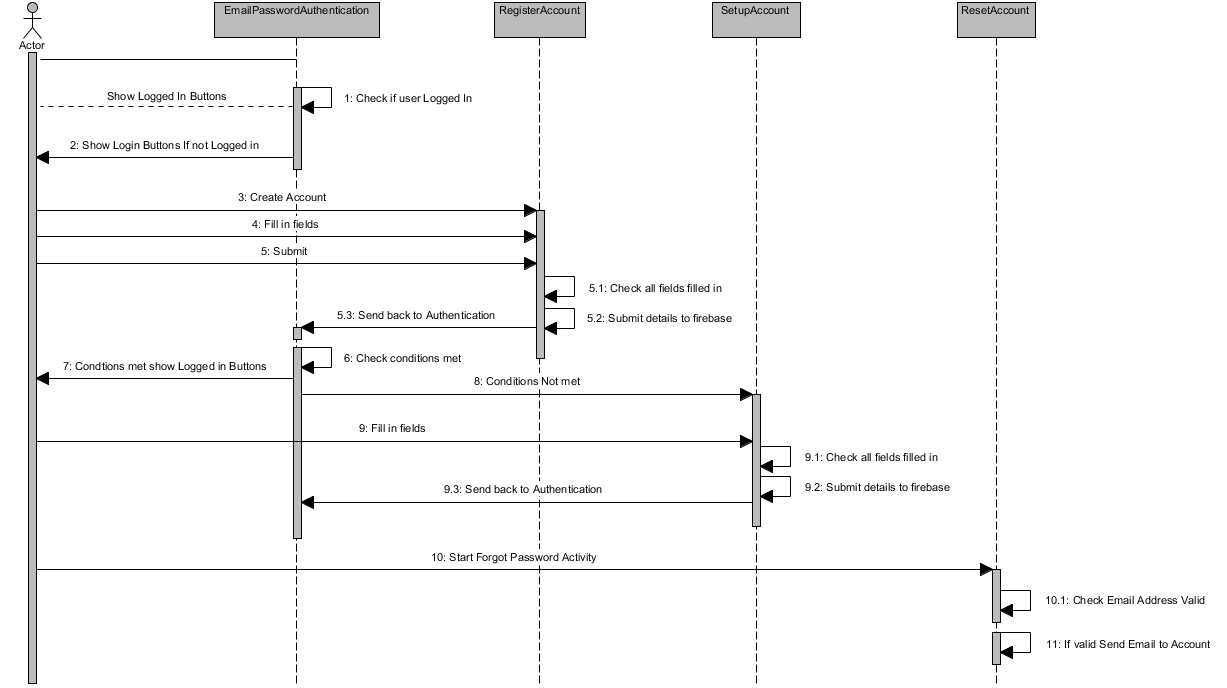
\includegraphics[width=500pt]{Login&RegisterSequence}\\
    \caption{Login Sequence Diagram } \label{Figure: Sequence Diagram}
\end{figure}

\par
While looking at the different activities on which the user may take there are also associated checks which need to be performed to proceed to the next area of the application. Even when a new user creates an account the following account needs to be verified with the Firebase database to check if such a user exists this is not just for authentication but to enable users to post their accurate information with an allocated name, profile picture and unique ID which distinguish's them from other users. When a user has either created an account by registering with an indifferent email address or signing in with the aid of Google sign in, on the authorization of the account The user is brought back to the EmailAndPasswordAuthentication Activity. On which the user is validated, and new options are then shown to the user for them to proceed to the MapActivity or to change preferences as well as signing out of the application.

\section{Maps and Geofencing Diagrams}
The following section is to show using diagrams how the maps and geofencing activity works and its associated classes and activities that are combined to retrieve notifications on which a user has entered a specific geofence. With hence to its specific class, the maps activity must have an allocated map fragment which is defined on the designed layout that is accessed by a reference by the class to produce a suitable map. On gaining the Location of the device we first need to check the permissions of the application especially if the device is using Android Marshmallow or above. As there are new permission intents on which the user must explicitly accept to use specific components of such device. When these permissions have been accepted the application then has access to the GPS module located in the device which most mobiles have in this day and age. With these specific settings turned on and with the permissions set in hand, the app is then available to accept location updates which are set on that activities class and are updated by specific intervals which are set by the developer. These are just a few of the methods that the developer will run through on the next chapter but for now the diagrams of communication between the user and device.

\subsection{Maps and Geofence Use Case Diagram}
While viewing the following use case diagram located in figure 5.6, the reader can see that it is quite an easy diagram to comprehend as there are only three use cases that can be seen on which the user can use with specific button clicks. The main area of this map activity is to utilise the GPS locator of the device to receive updates on whether the user has entered a geofence location which a notification and dialogue pop-up will appear to the user entering such an area.

\begin{figure}[htbp]
    \center 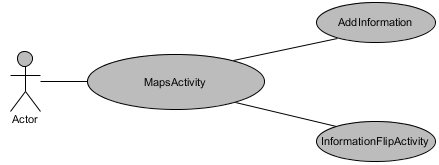
\includegraphics[width=450pt]{MapsUsecase}\\
    \caption{Maps \& Geofence Use Case Diagram } \label{Figure: Maps & Geofence Use Case Diagram}
\end{figure}

\subsection{Maps and Geofence Activity Diagram}
We can see by looking at the following diagram figure 5.7, on which how each specific component is mapped to the main MapsActivity which does all of the computation with regards to retrieving a location from the device which allows for this app to be a location aware application. While looking at the two reference classes and distinguishing what if anything they do is simple. The Place class utilises the notification thrown when a user is in a geofence. The maps activity acts as a broadcast receiver to retrieve the information which a pending notification intent was thrown populates the Place methods with the name of the area which a notification was thrown and passed to the InformationFrontActivity when the users choose to enter the specific monuments activity.\par

\begin{figure}[htbp]
    \center 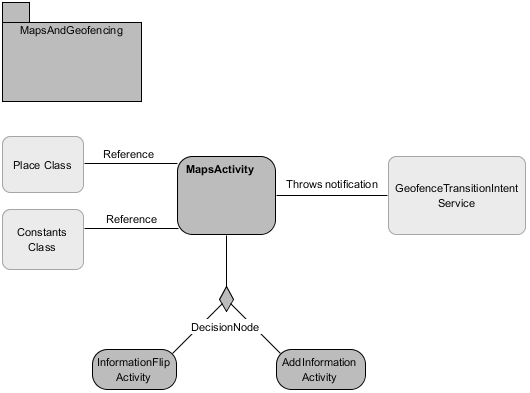
\includegraphics[width=450pt]{MapsGeofenceActivity}\\
    \caption{Maps \& Geofence Activity Diagram} \label{Figure: Maps & Geofence Activity Diagram }
\end{figure}
\newpage
\subsection{Maps and Geofence Sequence Diagram}
The following sequence diagram located in figure 5.8 represents the states of which the user will be initiated through with hence to the background workings of the application. While viewing the diagram, the reader can see the initial connection between the user and MapsActivity.  Which the onCreate of that specific activity triggers methods which set up the map fragment, adding geofences which are retrieved from firebase, GoogleApi which is needed to request the location from the user's devices as well as the connectors to the camera view to adjust the camera view of the map on location changes. With this in mind when the location changes the application renders whether the application has entered a geofence location. On going into a geofence, a pending intent will be initiated which will then trigger a notification which will display on the user's device. The user may want to view the information or not it is not compulsory to view the information on the application. Another opportunity on which a user might want to undertake is to send information to the InforMe@Dublin Gmail account to add more geofences with images and information to the InforMe@Dublin Android Application.\newpage

\begin{figure}[htbp]
    \center 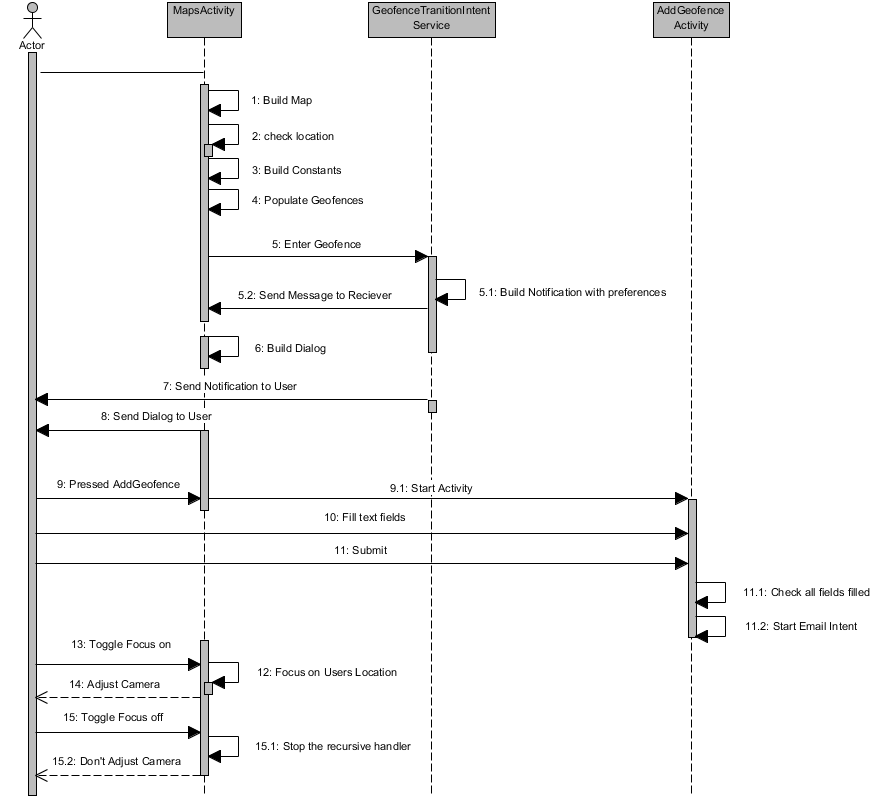
\includegraphics[width=400pt]{MapsSequence}\\
    \caption{Maps \& Geofence Sequence Diagram} \label{Figure: Maps & Geofence Sequence Diagram }
\end{figure}

\section{Information and Posting Diagrams}
During the following phase of the project is where the user can view the information of the monument on which they have entered and post some information about that specific area if they wish while they are in the same vicinity of the monument. These fragments which are created when the user selects to view the information on the specific area. On using the icons which change the view of each fragment activity when on the informationBackCommentsFragment is on the main view users can then choose to Post comments, update comments or just to view the post as a whole without other posts in the way. The following Diagrams will display how each component works together to retrieve information for where exactly the user is located.

\subsection{Information and Posting Use Case Diagram}
Regarding the following diagram figure 5.9 showing the use case diagram as shown distinguishes how each of the user's actions is mapped on clicking certain buttons which were applied to the layout file and linked to the activity. On entering the InformationFlipActivity, the user is sent to the InformationFrontFragment which displays the information of the monument of which the user has entered the specific geofence. The user can only access these specific activities on entering from an allocated geofence.\par

\begin{figure}[htbp]
    \center 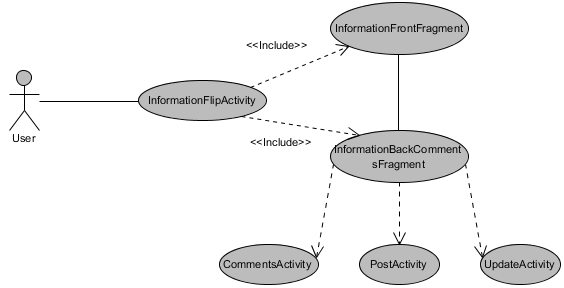
\includegraphics[width=350pt]{PostingAndInformationUsecase}\\
    \caption{Information \& Posting Use Case Diagram} \label{Figure: Information & Posting Use Case Diagram }
\end{figure}

\newpage

\subsection{Information and Posting Activity Diagram}
Regarding the Activity diagram in figure 5.10, the reader can see how each part of the package PostingInformationAndComments the classes as follows in the diagram. The InformationFlipActivity controls both InformationFrontFragment and InformationBackCommentsFragment both of these fragments are controlled using the menu bar of these fragments the InformationFlipActivity uses a stack to flip each of the fragments back to front. Only when the InformationBackCommentsFragment is displayed may the users create and view posts made by other users and also themselves When viewing the posts, the user can then like specific posts that have been created by the user or other users.\par

\begin{figure}[htbp]
    \center 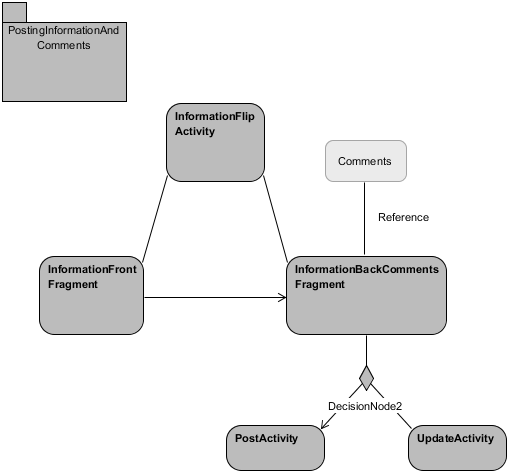
\includegraphics[width=350pt]{PostingInformation}\\
    \caption{Information \& Posting Activity Diagram} \label{Figure: Information & Posting Activity Diagram }
\end{figure}

\newpage

\subsection{Information and Posting Sequence Diagram}
Looking at the diagram in figure 5.11 the reader will grasp a better understanding of the following Activities on viewing the information of the specific monument as well as viewing the posts which are retrieved using firebase methods on which the developer will discuss in the following chapters. On entering the front fragment, the following methods are then initiated on starting the activity such as retrieving the information from the Firebase database which has been referenced to the specific JSON file. The fields of the activity will then be populated with the information which has been retrieved as well as images being loaded with specific URL's which have been saved in a hashmap and loaded within a page scroller. On viewing the posts from the user, these are populated by using the InformationBackCommentsFragment as well as the Comments class to populate the data and to display in a page view of specific user's posts which were posted on that monuments page.\par

\begin{figure}[htbp]
    \center 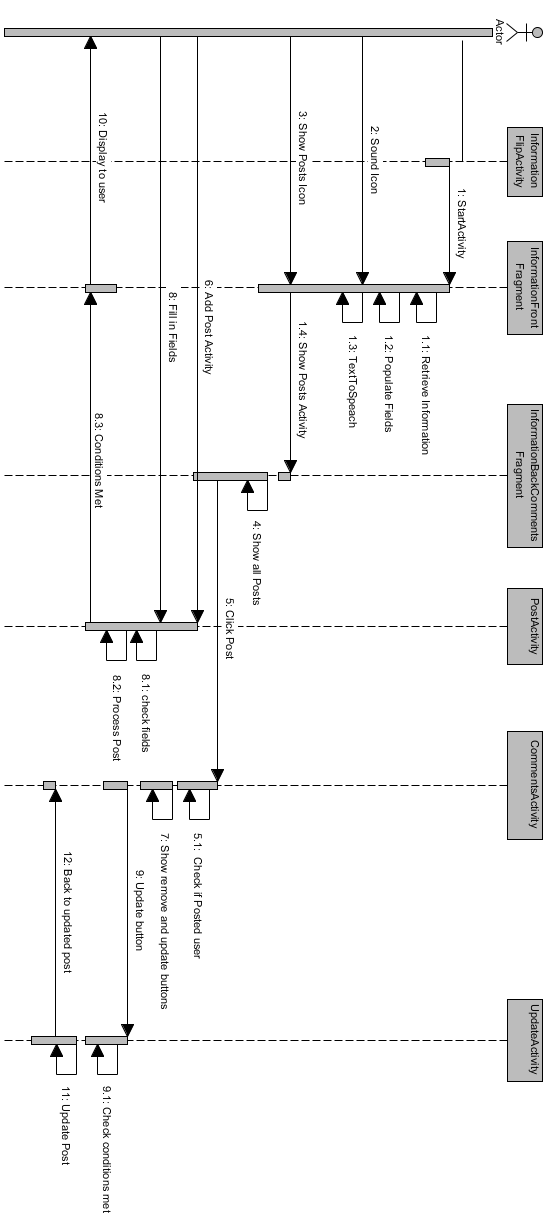
\includegraphics[width=250pt]{PostingAndInformationSequence}\\
    \caption{Information \& Posting Sequence Diagram} \label{Figure: Information & Posting Sequence Diagram }
\end{figure}

\newpage

\section{Settings Diagrams}
The following diagrams regarding the settings preferences are discussed throughout this section of the chapter. With hence to the settings activity, the user can change the application's preference with regards to setting the vibration of the notification which is sent on entering the geofence. The user can also change the notification sound as well as a battery save mode which utilises the proximity sensor to sense if the device's screen is on and if the sensor of the device is covered.

\subsection{Settings Use Case Diagram}
The following diagram shows the reader how the Settings and activities that are combined within the preference activities which allow the user to change specific settings for that application the user can change the settings as follows with the following activities as shown in the figure 5.12.\par

\begin{figure}[htbp]
    \center 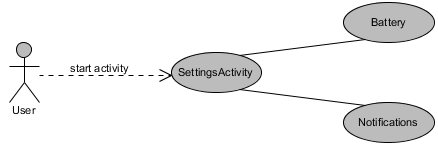
\includegraphics[width=450pt]{SettingsUsecase}\\
    \caption{Settings Use Case Diagram} \label{Figure: Settings Use Case Diagram }
\end{figure}

\subsection{Settings Activity Diagram}
The following diagram located in figure 5.13 shows the reader how the Settings and AppCompatActivity reference to each other when changing the preferences of the user. The CheckConnectivity class represents the application to see if the device is connected to the internet and if the Gps module is activated.

\begin{figure}[htbp]
    \center 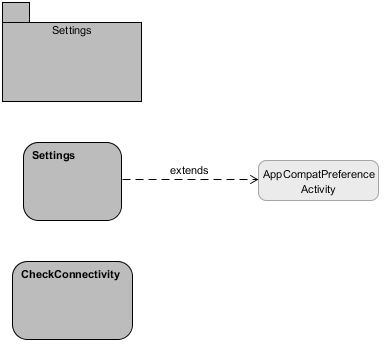
\includegraphics[width=350pt]{SettingsActivity}\\
    \caption{Settings Activity Diagram} \label{Figure: Settings Activity Diagram }
\end{figure}

\subsection{Settings Sequence Diagram}
While viewing the following diagram located in figure 5.14 shows how the user associates with the settings Activity while utilising the preference layouts as well as the AppCompatActivity this then shows the preference which will be discussed in the next chapter of this thesis. 

\begin{figure}[htbp]
    \center 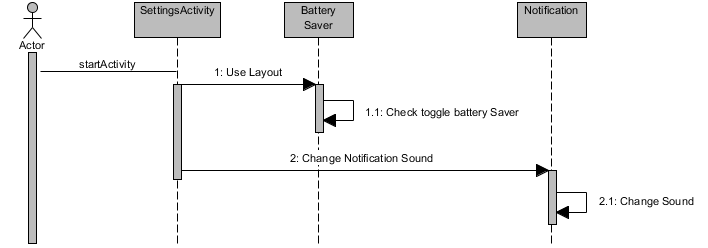
\includegraphics[width=450pt]{SequenceDiagramSettings}\\
    \caption{Settings Sequence Diagram} \label{Figure: Settings Sequence Diagram }
\end{figure}

\section{Overall System Use Case Diagram}
The following diagram represents the InforMe@Dublin application as a whole. Concerning the following use case diagram located in figure 5.15, the reader can then see all of the different components on which a user can enter within the constraints of being signed in and with the submission of posts by the specific user being able to remove and update their specific posts. The reader can see how each component is connected to each other and on where the user can gain access to certain activities throughout the following application.\par

\begin{figure}[htbp]
    \center 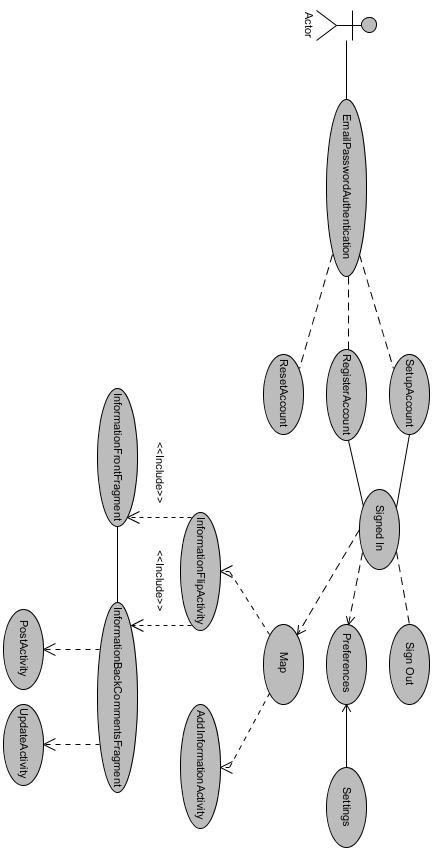
\includegraphics[width=300pt]{FullActivityUseCase}\\
    \caption{Overall Use Case Diagram} \label{Figure: Overall Use Case Diagram }
\end{figure}

\newpage

\section{Activity Diagram with Overall System}
Regarding the diagram figure 5.16, The activity diagram as a whole is to show the reader how each component is used throughout the system to grasp a better understanding of which Activities and classes are working and what exactly is each of these specific items doing throughout the Android application. When brought together as a whole with descriptions of each package and the associated classes and activities the reader may gain a better understanding of the following project. The InforMe@Dublin Android application is not meant to be complex in nature but descriptive enough to show the findings the developer designed within the application.

\begin{figure}[htbp]
    \center 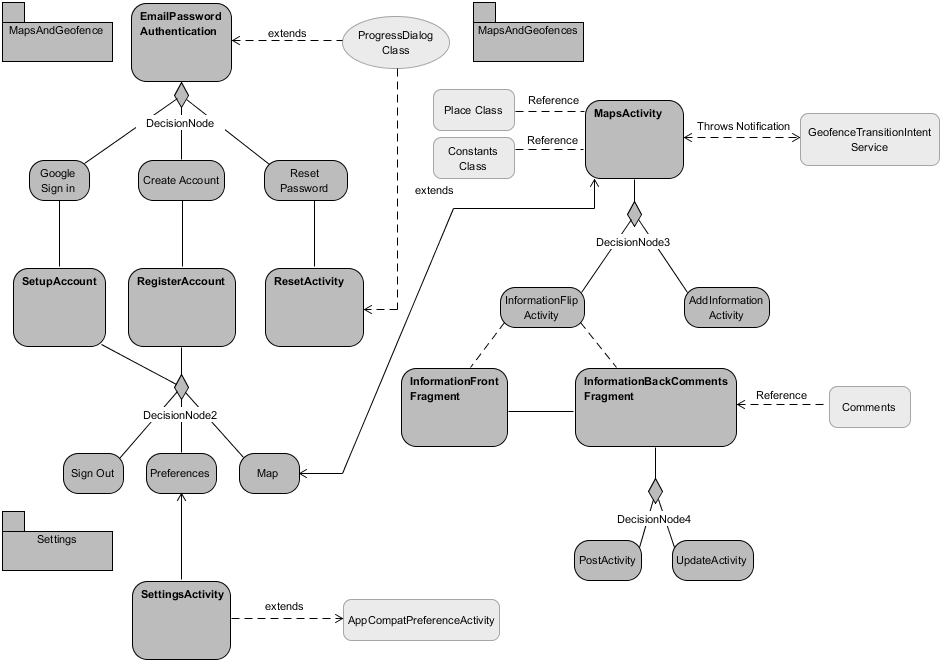
\includegraphics[width=470pt]{FullActivity}\\
    \caption{Overall Use Case Diagram} \label{Figure: Overall Activity Diagram }
\end{figure}


\section{Summary of the Chapter}
Throughout the following chapter, the developer has brought us through the different steps of how the user can interact with the application as a whole, and of which components of the app are connected to one another. Another aspect that the developer has to show us is the communication between the application within the packages of which are of a modular concern to the specific components of the app, concerning the MapsAndGeofence package holds all the classes and activities which are only used once a patron of the application is in that specific activity. With that in mind, the developer hopes that the reader understands how the application is mapped out and thoroughly understands of which the developer is trying to achieve. The next chapter of the following thesis is to show the wireframing and design aspects of the InforMe@Dublin Android application with hence to colour schemes and layouts of each specific activity.
